%% LaTeX2e class for student theses
%% sections/evaluation.tex
%% 
%% Karlsruhe Institute of Technology
%% Institute for Program Structures and Data Organization
%% Chair for Software Design and Quality (SDQ)
%%
%% Dr.-Ing. Erik Burger
%% burger@kit.edu
%%
%% Version 1.3.2, 2017-08-01

\chapter{Evaluation on Reverberated Data}
\label{ch:results}
This section contains the final evaluation. It describes how different models performed on reverberated data.
\section{Neural Network Models}
We compare the four-layer TDNN model with a fully connected baseline model that was also used in \cite{nguyen20162016}. 
\subsection{TDNN Model}
The TDNN model, which can be seen in figure \ref{fig:final_tdnn} is based on the results found in chapter \ref{ch:tdnn_design}. \\ 
\begin{minipage}{\linewidth}
	\vspace{5mm}
	\begin{tikzpicture}[x=1.8cm, y=1.5cm]
	% Input layer
	\node[text width=3cm] at (-1,0) {Input ($23*40$)};
	\foreach \m in {2,3,...,22}
	\node [tdnn neuron] (input-\m) at (\m*0.25,0) {};
	
	\node [tdnn neuron, label=below:$x_{t - 13}$] (input-1) at (1*0.25,0) {};
	\node [tdnn neuron, label=below:$x_{t + 9}$] (input-23) at (23*0.25,0) {};
	
	% TDNN 1
	\node[text width=3cm] at (-1,0.5) {TDNN/LP 1};
	\node[text width=3cm] at (-1,1) {Hidden ($7*300$)};
	\foreach \m [count=\y] in {1,2,...,7}
	\node [tdnn neuron] (hidden-1-\m) at (\y*0.25*3,1) {};
	
	% Splice
	\node[text width=3cm] at (-1,1.5) {Splice};
	\node[text width=3cm] at (-1,2) {Hidden ($8*300$)};
	\foreach \m [count=\y] in {1,2,...,8}
	\node [tdnn neuron] (hidden-2-\m) at (\y*0.25*3 - 0.40,2) {};
	
	% TDNN 2
	\node[text width=3cm] at (-1,2.5) {TDNN/LP 2};
	\node[text width=3cm] at (-1,3) {Hidden ($4*300$)};
	\foreach \m [count=\y] in {1,2,...,4}
	\node [tdnn neuron] (hidden-3-\m) at (\y*0.25*6 - 0.80,3) {};
	
	% TDNN 3
	\node[text width=3cm] at (-1,3.5) {TDNN/LP 2};
	\node[text width=3cm] at (-1,4) {Hidden ($2*300$)};
	\foreach \m [count=\y] in {1,2}
	\node [tdnn neuron] (hidden-4-\m) at (\y*0.25*12 - 1.60,4) {};
	
	% TDNN 4
	\node[text width=3cm] at (-1,4.5) {TDNN/LP 2};
	\node[text width=3cm] at (-1,5) {Hidden ($1*400$)};
	\node [tdnn neuron] (hidden-5) at (1*0.25 + 11 * 0.25,5) {};
	
	% Classifier
	\node[text width=3cm] at (-1,5.5) {Linear/Softmax};
	\node[text width=3cm] at (-1,6) {Output ($1*8156$)};
	\node [tdnn neuron, label=above:$y_{t}$] (classify-1) at (1*0.25 + 11 * 0.25,6) {};
	
	% Edges
	%L1 Edges
	\foreach \m [
	evaluate=\m as \nstart using int(((\m - 1) * 3) + 1),
	evaluate=\m as \nstep using int(((\m - 1) * 3) + 2),
	evaluate=\m as \nend using int(((\m - 1)* 3) + 5)] in {1,2,...,7}
	\foreach \i in {\nstart,\nstep,...,\nend}
	\draw (input-\i.north) -- (hidden-1-\m);  
	
	%Splice Edge
	\draw (hidden-1-1.north) -- (hidden-2-1.south);  
	\draw (hidden-1-2.north) -- (hidden-2-2.south);
	\draw (hidden-1-3.north) -- (hidden-2-3.south);
	\draw (hidden-1-4.north) -- (hidden-2-4.south);
	\draw (hidden-1-4.north) -- (hidden-2-5.south);
	\draw (hidden-1-5.north) -- (hidden-2-6.south);
	\draw (hidden-1-6.north) -- (hidden-2-7.south);
	\draw (hidden-1-7.north) -- (hidden-2-8.south);
	
	% Edges
	%L2 Edges
	\foreach \m [
	evaluate=\m as \na using int(((\m - 1) * 2) + 1),
	evaluate=\m as \nb using int(((\m - 1) * 2) + 2)] in {1,2,...,4} {
		\draw (hidden-2-\na.north) -- (hidden-3-\m);
		\draw (hidden-2-\nb.north) -- (hidden-3-\m);
	}
	
	%Edges
	%L3 Edges
	\draw (hidden-3-1.north) -- (hidden-4-1);
	\draw (hidden-3-2.north) -- (hidden-4-1);
	\draw (hidden-3-3.north) -- (hidden-4-2);
	\draw (hidden-3-4.north) -- (hidden-4-2);
	
	%L4 edges
	\draw (hidden-4-1) -- (hidden-5);
	\draw (hidden-4-2) -- (hidden-5);

	% Classify Edges
	\draw (hidden-5) -- (classify-1);
	
	\end{tikzpicture}
	\captionof{figure}{Illustration of the final TDNN model in the time domain}
	\label{fig:final_tdnn}
	\vspace{5mm}
\end{minipage}\\ \\
It consists of four TDNN layers and one linear layer at the end, followed by a softmax nonlinearity. After each TDNN layer, a L2 pooling nonlinearity with zeroing of unstable gradients and a pool size of ten is used. A splicing layer with the splicing configuration $(0, 1, 2, 3, 3, 4, 5, 6)$ was used after the first TDNN layer. The exact configuration of kernel sizes and strides can be found in table \ref{tbl:tdnn_layer_design}. The output of each TDNN layer had 3000 channels, the output of each pooling layer 300 channels. The input context consisted was $(-13, 9)$. The count of channels, the modified L2 pooling gradient and the omission of batch normalization was the main difference to the architecture described in \cite{peddinti2015reverberation} and \cite{peddinti2015jhu}. 
\subsection{Fully Connected Baseline Model}
We compare the results of our TDNN with a fully connected network that achieved comparable performance on an reverberated training set. The model consists of six linear layers with a width of 1600, followed by ReLU nonlinearities. The output layer is a linear layer followed by a Softmax nonlinearity. We tested input contexts of $(-13, 9)$ as well as $(-5, 5)$.
\section{Training Setup}
We used the same training set as described in chapter \ref{ch:tdnn_design} as well as a reverberated version of the training set. As in chapter \ref{ch:tdnn_design}, we used a SGD variant with newbob learning rate scheduling and momentum. The loss function was frame based cross entropy loss. The input features at each time frame were 40 log-mel coefficients as in \cite{nguyen20162016}. Our input features were mean normalized over the whole utterance with a mean of zero and a variance of two. This is different from the unnormalized 140 dimensional input vector used by \cite{peddinti2015reverberation} in \cite{peddinti2015jhu} for their TDNN model.
\section{Data Augmentation}
For training and evaluating acoustic models that are robust on reverberated data, we trained them on data that was reverberated as well. For this purpose, we used a collection of recorded room impulse responses to augment our data set. This follows the theoretical insight given in section \ref{sec:reverberation}: For each audio sequence in our data set, we pick a random room impulse response and convolute the two signals to from an augmented signal. \\ \\
The room impulse responses we used are similar as in \cite{ritter2016training}. However we did only use the RWCP \cite{nakamura2000acoustical}, OMNI \cite{stewart2010database} and ACE \cite{eaton2015ace} datasets. The AIR dataset  \cite{jeub2009binaural} was not used, since the amplitude in the different recordings in the dataset change significantly.
Evaluating the effects of different signal amplitudes was not a goal of this work, as we can assume that the audio frontend used will always provide a reasonable gain. We therefore normalized the room impulse responses very carefully before performing the convolution based on their signal energy. For the ACE dataset, we found that the energy direct transmission path was very low compared to the noise. In this case, we amplified the direct transmission path to generate a meaningful result.
Illustration \ref{fig:air_spectrogram} shows an audio sample that was reverberated with this method. 
\section{Evaluation Results}
We test the four-layer TDNN model with the input context $(-13, 9)$, as well as the fully connected (\textit{FC}) model with the input contexts $(-13, 9)$ and $(-5, 5)$. To do so, we train each model on the clean training set as described in chapter \ref{ch:tdnn_design}. We separately tune each model on a combination on the clean and reverberated training set, with a total length of 902~hours. Then, we tune the $l_p$, $l_z$, master beam and softmax temperature parameters using the development set mentioned in chapter \ref{ch:tdnn_design}. The development set was not augmented. \\ \\ Since was impossible to fit the combined 902~hour dataset entirely into memory, and loading from disk was very slow with the large input context of $(-13, 9)$, we reduced the precision of the training dataset to 16~bits for all experiments in this section. We validated this approach by also running several experiments different on the clean dataset with the original precision. The differences in terms of FER were below 0.1\% where sometimes the model trained on high precision and sometimes a model low precision was better. In terms of WER we did not observe any difference on the development set. \\ \\
For this evaluation we use the \textit{tst2014} dataset, which was the evaluation dataset for the IWSLT 2014 conference \cite{cettolo2014report}. Similar to our development dataset, the evaluation dataset also consists of TED talks with a total length of 2.1~hours. \\ \\
The TDNN model, which has 4.2~million parameters, trained for 14~epochs, where each epoch took 9.3~hours on the combined dataset, on a single GTX~1080~Ti~GPU. On the clean dataset, a single training epoch took 4.2~hours. The fully connected models with short and long input contexts had 13.2~million and 13.6~million parameters respectively. They trained for 12 and 11 epochs, where each epoch took 1.3~hours on the clean dataset and 2.3~hours on the combined dataset. 
\\ \\
The results of our evaluation can be seen in figure \ref{fig:final_validation}. For models trained on clean data, the word error rate on the reverberated development set is high. It can be seen that models with larger input context performed better on unseen reverberated data. On the clean validation set, all models performed similar. \\ \\
\begin{minipage}{\linewidth}
\begin{minipage}{\linewidth}
\centering
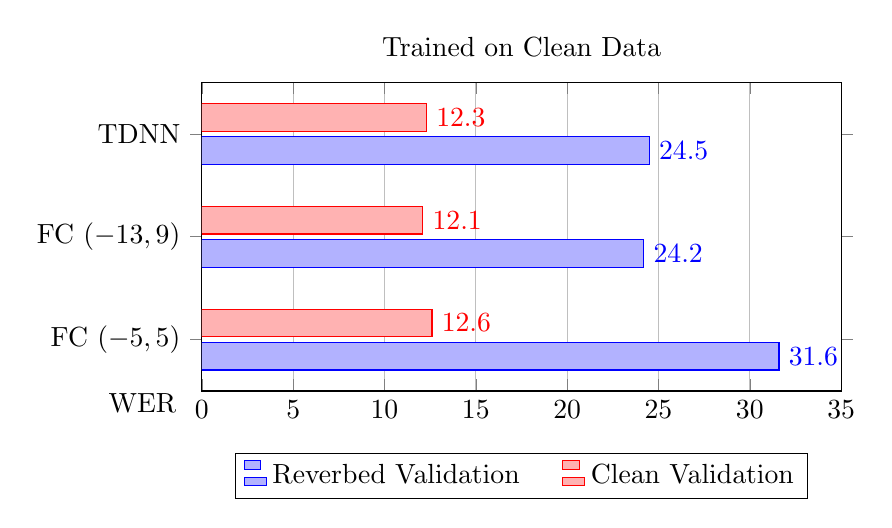
\begin{tikzpicture}
\begin{axis}[
title=Trained on Clean Data,
xbar,xmajorgrids=true,
width=0.8\linewidth,height=5.5cm, enlarge y limits=0.25,
xmin=0,xmax=35,xlabel={WER},xlabel style={
	at={(ticklabel cs:0)},
	anchor=north east,
	yshift=0.56 cm, xshift=-0.2cm
},
symbolic y coords={FC \text{$(-5,5)$}, FC \text{$(-13,9)$}, TDNN},
ytick=data,nodes near coords, nodes near coords align={horizontal},
legend style={at={(0.5,-0.2)},
	anchor=north,legend columns=2}
]
\addplot coordinates {(31.6,FC \text{$(-5,5)$}) (24.2,FC \text{$(-13,9)$}) (24.5,TDNN)};
\addlegendentry{Reverbed Validation \quad \quad}
\addplot coordinates {(12.6,FC \text{$(-5,5)$}) (12.1,FC \text{$(-13,9)$}) (12.3,TDNN)};
\addlegendentry{Clean Validation}
\end{axis}
\end{tikzpicture}
\end{minipage}
\\ \\ \\ 
\begin{minipage}{\linewidth}
\centering
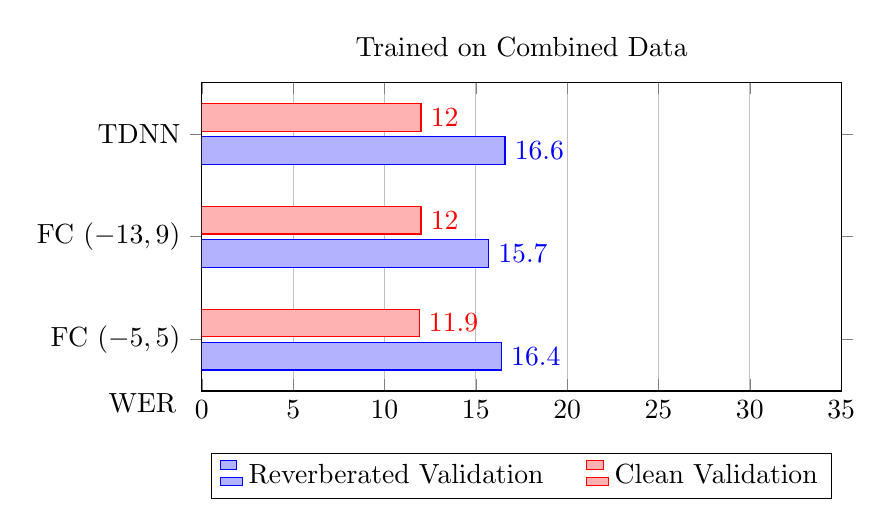
\begin{tikzpicture}
	\begin{axis}[
	title=Trained on Combined Data,
	xbar,xmajorgrids=true,
	width=0.8\linewidth,height=5.5cm, enlarge y limits=0.25,
	xmin=0,xmax=35,xlabel={WER}, xlabel style={
       at={(ticklabel cs:0)},
	   anchor=north east,
	   yshift=0.56 cm, xshift=-0.2cm
	},
	symbolic y coords={FC \text{$(-5,5)$}, FC \text{$(-13,9)$}, TDNN},
	ytick=data,nodes near coords, nodes near coords align={horizontal},
	legend style={at={(0.5,-0.2)},
		anchor=north,legend columns=2}
	]
	\addplot coordinates {(16.4,FC \text{$(-5,5)$}) (15.7,FC \text{$(-13,9)$}) (16.6,TDNN)};
	\addlegendentry{Reverberated Validation \quad \quad}
	\addplot coordinates {(11.9,FC \text{$(-5,5)$}) (12,FC \text{$(-13,9)$}) (12,TDNN)};
	\addlegendentry{Clean Validation}
	\end{axis}
	\end{tikzpicture}
	\captionof{figure}{Word Error Rate on the clean and reverberated validation dataset for models trained on clean and combined training data, respectively}
	\label{fig:final_validation}
\end{minipage} 
\end{minipage} 
\\ \\ \\
For models trained on reverberated data, the performance on reverberated validation is similar data for all three models. The same holds for clean validation data. The fully connected model with a large input context outperformed the other models on the reverberated validation set by a small margin. All models performed slightly better on clean validation data than the same model trained on clean data only, where the difference was most significant for the fully connected model with short input context. \\ \\
From this observations we conclude that data augmentation can be sufficient for improving acoustic model performance for reverberated audio. A larger input context can improve the robustness of the acoustic model in some cases. 
\iffalse
TODO: Describe how we generated reverbed data
TODO: Describe how we tested on reverbed data
TODO: Describe final architecture and results

This chapter should summarize and interpret the results. It should give a clear insight
about which methods did decrease the FER and WER on reverbed and unreverbed data, respectivley.
\fi